\part{Modelling systems using logic}
\setcounter{section}{0}

\newcommand{\atomr}{\textsf{r}}
\newcommand{\atomrp}{\textsf{r'}}
\newcommand{\atomg}{\textsf{g}}
\newcommand{\atomgp}{\textsf{g'}}

In this part we are going to briefly cover using propositional
formula to model systems. This is a common approach in hardware design
where a complete or partial model of a circuit or processor is defined in logic,
against which specifications of particular properties are checked.
The starting point is to work out a good way to represent/model a
system as a logical formula. In this part of the course, we will
consider systems modelled as simple state machines, with states and
transitions between the states describing how a system can
change/evolve. We will then convert this model into a propositional
formula.


To verify a system based on its model we then need a specification of
either good behaviour that we want to make sure follows from our model
or of bad behaviour which we want to ensure does not follow from the
model.  We formulate such a specification as a propositional formula
\emph{spec}, and then prove that the following is valid:
%
\begin{equation*}
\emph{model} \rightarrow \emph{spec}
\end{equation*}
%
The use of implication means that if the model holds then
the specification must hold. Alternatively, and equivalently,
we could state this as judgment $\emph{model} \vdash \emph{spec}$,
\ie{}, the specified behaviour follows from the model.

\section{State-transition models as propositions}

\paragraph{States}
Our running example will be a very simple traffic light comprising
a red light and a green light, with two possible states:
%
\setlength{\tabcolsep}{0.4em}
\begin{center}
  \begin{tabular}{m{1.1cm} m{1.5cm} m{1.1cm}}
    State 1 & & State 2 \\
{\scalebox{0.2}{
\includegraphics{images/red-on.pdf}}}
  &
  &
{\scalebox{0.2}{
\includegraphics{images/green-on.pdf}}}
\end{tabular}
\end{center}
%
Either the red light is on (left) or the green light is on (right),
but never both at the same time, and there is always at least one
light on. We will use two atoms (propositional
variables that can be true or false) $\atomr{}$ and $\atomg$ to represent the state of
each light separately, where:
%
\begin{itemize}
  \item \atomr{} means the red light is on; $\neg\atomr{}$ therefore
  means the red light is off;
  \item \atomg{} means the green light is on; $\neg\atomg{}$ means the
  green light is off.
\end{itemize}
%
The two valid states of the system can then be modelled as two propositions:
%
\begin{align*}
  \text{State 1} & \qquad\qquad \text{State 2} \\
  \atomr{} \wedge \neg\atomg{} &
  \qquad\qquad
  \neg\atomr{} \wedge \atomg{}
\end{align*}
%
For $n$-propositional atoms there are $2^n$ possible states that can
be modelled. Thus in our model, there are four possible states, two of
which we want to treat as valid (the above two).

\begin{exc}
Define a propositions for each of the two invalid states in the
traffic light.
\end{exc}

\noindent
\textbf{State transitions} \hspace{0.5em} So far we have modelled the states as propositions, but we also want to
model the behaviour of the system in terms of the possible
transitions between states. We can represent this
with a simple diagram:
%
\setlength{\tabcolsep}{0.4em}
\begin{center}
  \begin{tabular}{m{1.1cm} m{1.5cm} m{1.1cm}}
       State 1 & & State 2 \\[-0.5em]
{\scalebox{0.2}{
\includegraphics{images/red-on.pdf}}}
  &
    \xymatrix{
    \ar[rr]^{\textit{\normalsize{go}}} & & \\
     & & \ar[ll]^{\textit{\normalsize{stop}}}
    }
  &
{\scalebox{0.2}{
\includegraphics{images/green-on.pdf}}}
\end{tabular}
\end{center}
%
\ie{}, when just the red light is on it is possible to
transition to a state with just the green light on, and back again.

To model state transitions we will introduce two additional atoms
that model the future state of the lights in the system:
%
%
\begin{itemize}
\item \atomrp{} for the red light being on in the \emph{next time step};
\item \atomgp{} for the green light being on in the \emph{next time step}.
\end{itemize}
%
We can now express the above two transitions as implications:
%
\begin{align*}
  (\textit{go}) : \qquad & \atomr{} \wedge \neg\atomg{} \; \rightarrow \;
                           \neg\atomr{}' \wedge \atomg{}' \\
  (\textit{stop}): \qquad & \neg\atomr{} \wedge \atomg{} \; \rightarrow \;
                            \atomr{}' \wedge \neg\atomg{}'
\end{align*}
%
Said another way, (\textit{go}) defines that if State 1 is true now
we can move to State 2 in the future (in the ``next'' time step of the
system), and (\textit{stop}) conversely defines that if State 2 is
true now we can move to State 1 in the future.

We can now describe the full transition behaviour of the system as
the conjunction of the above two formula:
%
\begin{equation*}
\textit{model} =
(\atomr{} \wedge \neg\atomg{} \; \rightarrow \; \neg\atomr{}' \wedge
\atomg{}')
\, \wedge \,
(\neg\atomr{} \wedge \atomg{} \; \rightarrow \; \atomr{}' \wedge \neg\atomg{}')
\end{equation*}
%
This provides our model of the system. You might be wondering why we
don't add more to this, \eg{}, ruling out invalid states. We will come
back to this point in Section~\ref{subsec:whenisamodelgood}.

% TODO: guiding principles, why not and this with the valid states?
% want to make a small formula and this follows
% need to come back to this?

\paragraph{A general approach}

The general approach to modelling a system in this way is to:
%
\begin{itemize}
  \item Decide what to represent about the state space of the system
  and introduce propositional atoms for these components.
  \item Model future states using ``next step'' atoms (usually written with
  an apostrophe, and called the ``primed'' atoms, \eg{}, \atomrp{} is
  read as ``r prime'').
 \item Write a propositional formula \emph{model} using these
  variables which takes the conjunction of state transitions expressed
  as implications.
\end{itemize}

\begin{exc}
Write down a model for a more realistic traffic light, \ie{}, that can
be described by the following states and transitions:
%

\begin{center}
\scalebox{0.28}{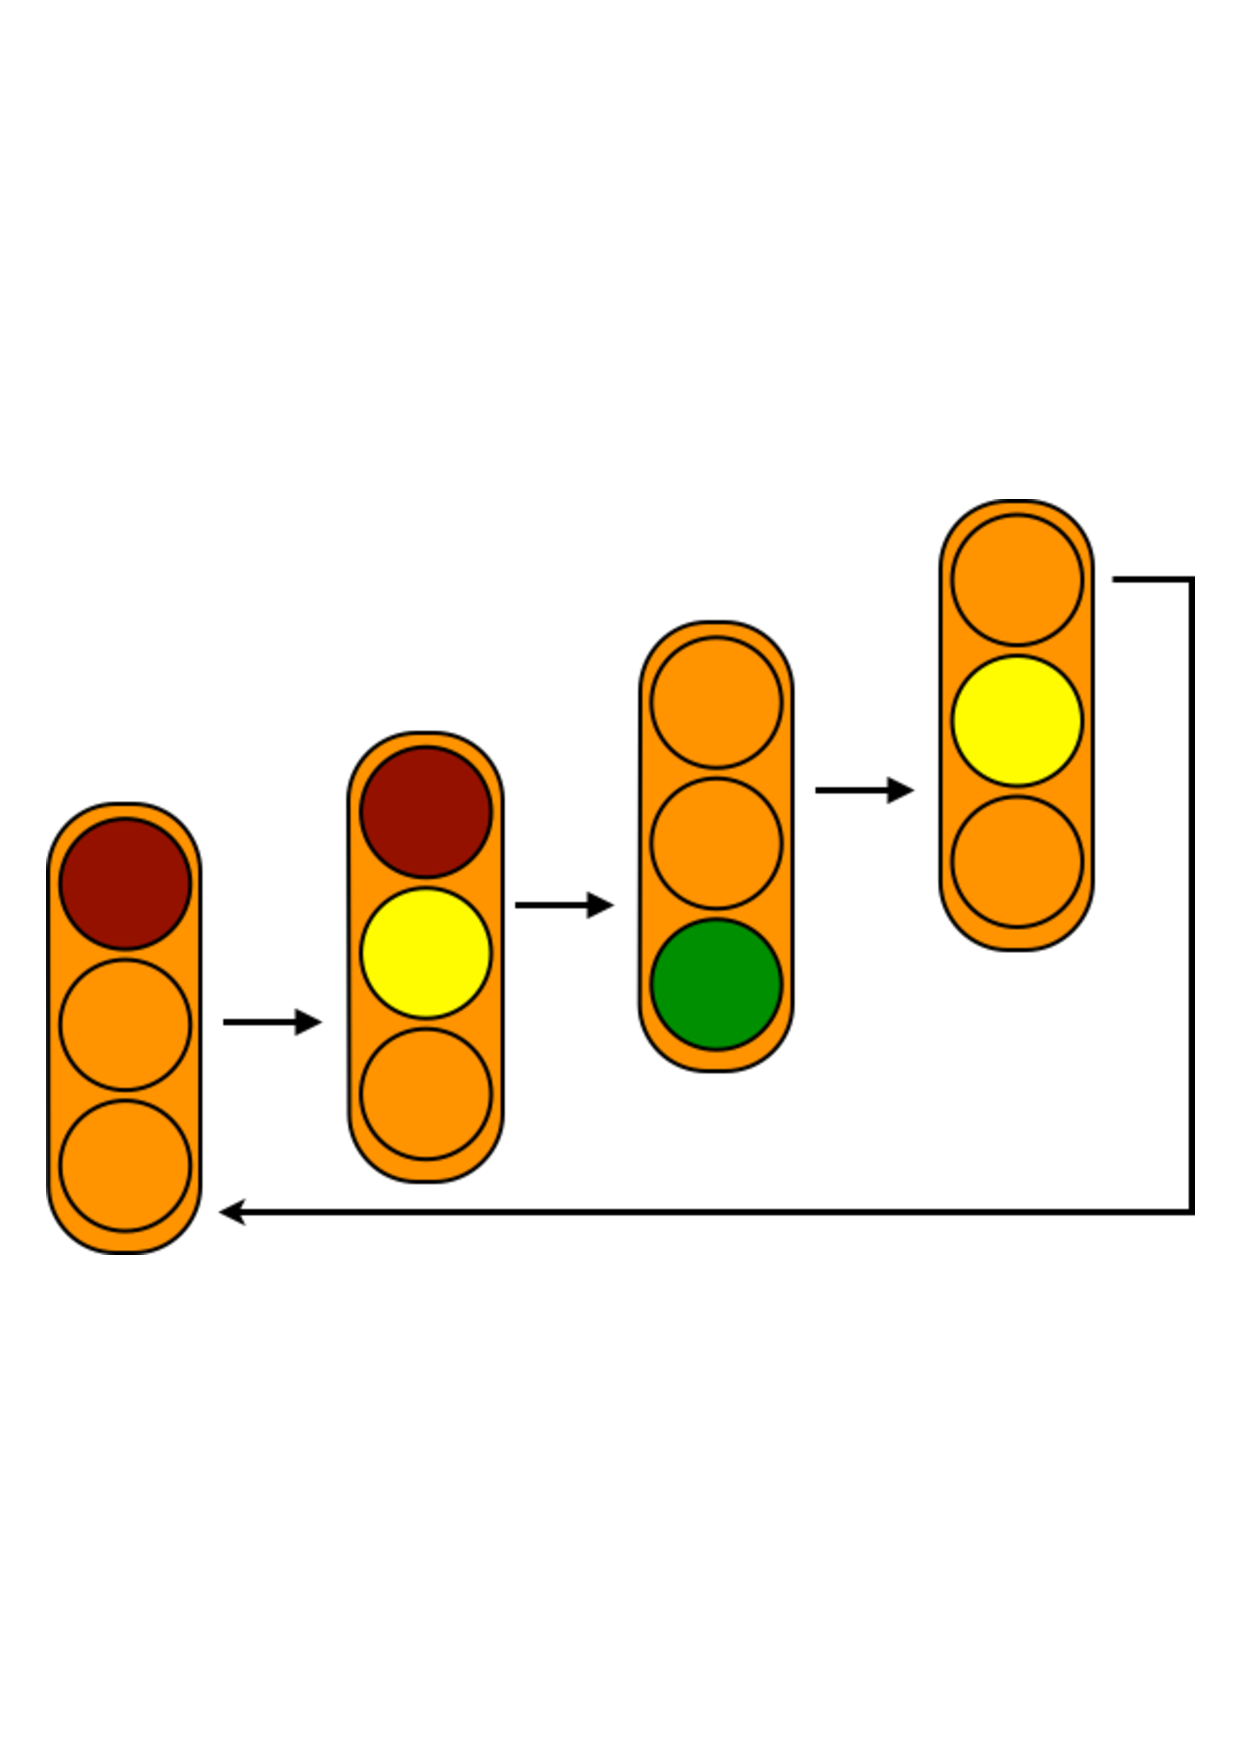
\includegraphics{images/full-light.pdf}}
\end{center}
\end{exc}

\section{Defining specifications as propositions}
\label{sec:spec}

Consider the following property which we might want to check
for our system:
%
\begin{quote}
\emph{If we are in a valid state and change state, then our new state
  is also valid.}
\end{quote}
%
We can abstract the notion of a valid state with the following
meta-level operation (you can think of this as a syntax function mapping from the
two propositions to a proposition):
%
\begin{equation*}
\textsf{valid-state}(r, g) = (r \wedge \neg g) \vee (\neg r \wedge g)
\end{equation*}
%
From this, we can then capture our specification as the proposition:
%
\begin{equation*}
  \textit{specification} = \textsf{valid-state}(\atomr, \atomg)
  \rightarrow \textsf{valid-state}(\atomrp, \atomgp)
\end{equation*}
%
\ie{}, a valid state now implies a valid state in the next time step.
To verify that our system (based on its model) satisfies this
property, we then need to prove that the following is true:
%
\begin{align*}
 & \textit{model} \rightarrow \textit{specification} \\
  \equiv \; &
((\atomr{} \wedge \neg\atomg{} \; \rightarrow \; \neg\atomr{}' \wedge
\atomg{}')
\wedge
(\neg\atomr{} \wedge \atomg{} \; \rightarrow \; \atomr{}' \wedge
  \neg\atomg{}'))
  \rightarrow
   (\textsf{valid-state}(\atomr, \atomg)
           \rightarrow \textsf{valid-state}(\atomrp, \atomgp)) \\
  \equiv \; &
((\atomr{} \wedge \neg\atomg{} \; \rightarrow \; \neg\atomr{}' \wedge
\atomg{}')
\wedge
(\neg\atomr{} \wedge \atomg{} \; \rightarrow \; \atomr{}' \wedge
  \neg\atomg{}'))
              \rightarrow
              (((\atomr \wedge \neg \atomg) \vee (\neg \atomr \wedge \atomg))
              \rightarrow ((\atomrp \wedge \neg \atomgp) \vee (\neg \atomrp \wedge \atomgp)))
\end{align*}
%
This is quite a big proposition so we might not want to prove it by
hand. Instead, in the next part of the course we are going to use an
algorithmic technique for proving that this holds (Part C,
specifically \textbf{Example 5} in the notes). We will later see that
this does indeed hold, and thus the system (as described by the model)
satisfies our specification.


\section{When is a model a good model?}
\label{subsec:whenisamodelgood}

\begin{quote}
\emph{All models are wrong but some are useful} (Box, 1978)
\end{quote}

\noindent
Indeed, a model is necessarily ``wrong'' in the sense that a model
abstracts some of the details of a real system; we are not
capturing every aspect of the system, such as: how are the transitions
triggered? or, what happens if a car crashes into the traffic light? Some
models, though eliding details, are useful in the sense that we
can detect when the system does not behave according to our
specification or we can verify that it always behaves according to our
specification. Just enough detail is needed in the model to capture what
we want to prove.

Our running example has the model:
\begin{equation*}
\mathit{model} =
(\atomr{} \wedge \neg\atomg{} \; \rightarrow \; \neg\atomr{}' \wedge
\atomg{}')
\wedge
(\neg\atomr{} \wedge \atomg{} \; \rightarrow \; \atomr{}' \wedge \neg\atomg{}')
\end{equation*}
%
We might add to this model the explicit exclusion of invalid
states. Let's define the condition of the invalid states via the meta-level function:
%
\begin{equation*}
\textsf{invalid-state}(r, g) = (\neg r \wedge \neg g) \vee (r \wedge g)
\end{equation*}
%
Then we could define an alternate model as:
%
\begin{equation*}
\mathit{model2} = \mathit{model} \wedge \neg \textsf{invalid-state}(\atomr, \atomg)
\end{equation*}
%
Thus, the new model adds to the old model that the current state is not
invalid.

In the case of the proving our specification from
Section~\ref{sec:spec} (that valid states transition to valid states)
we do not need this additional detail in the model. But we might want
to have this more restrictive model if we want to prove, for example,
that we can never be in an invalid state, regardless of what state we
started from. This can be captured by the new specification:
%
\begin{equation*}
\mathit{specification2} = \textsf{invalid-state}(\atomr, \atomg)
\vee \textsf{invalid-state}(\atomr', \atomg')
\end{equation*}
%
and proving that the following proposition is valid:
$$
\mathit{model2} \rightarrow
\neg \mathit{specification2}
$$
Note we are using a negative property
here: we show that the new model (\textit{model2}) implies that the bad behaviour is not possible.
For the old model (\textit{model}), a similar proposition capturing the same idea is valid:
$$
\mathit{model} \rightarrow \neg \mathit{specification2}
$$
However, the following proposition is also valid!!!
$$
\mathit{model} \rightarrow \mathit{specification2}
$$
Why? If the right-hand side of the implication is true (we have an
invalid state) the left-hand side is still true (the premise of each
transition implication is false, therefore the implications are
trivially true); the original model never excludes invalid states on
their own, only as the result of a transition from a valid
state. Thus, the original model was not a good model for checking the
$\mathit{specification2}$ property, but it was sufficient for
$\mathit{specification}$.

Creating a rich enough model is up to you, and requires some care and
thought about the domain and what properties are of interest.

\part{Natural deduction for first-order logic}
\setcounter{section}{0}

First-order logic quantifiers have natural deduction elimination and introduction rules.

\section{Introducing and eliminating quantifiers}

\subsection{Universal quantification $\forall$ (\emph{for all})}

The notion that universals generalise conjunction
($\forall x . P = P[a_0/x] \wedge P[a_1/x] \wedge
\ldots \wedge P[a_{n}/x]$, \S\ref{subsec:quantifier-meaning})
helps to understand the elimination and introduction rules of universal
quantification.

\paragraph{Elimination} As a reminder, here
are the conjunction elimination rules:
%
\begin{equation*}
\dfrac{P \wedge Q}
        {P} \; {\wedge_{e1}}
\;\;
\dfrac{P \wedge Q}
  {Q} \; {\wedge_{e2}}
\end{equation*}
%
We could apply these two
rules repeatedly to get any formula out of the conjunction
$P[a_0/x] \wedge P[a_1/x] \wedge
\ldots \wedge P[a_{n}/x]$, giving us the following inference for
the $i^{th}$ part of the conjunction:
%
\begin{equation*}
  \dfrac{P[a_0/x] \wedge P[a_1/x] \wedge \ldots \wedge P[a_{n}/x]}
  {P[a_i/x]}
\end{equation*}
%
This is essentially how we do universal quantification elimination.
Universal quantification differs to conjunction in that each one of the things
being ``conjuncted'' together is of the same form: they are all $P$
with some variable $x$ replaced by an element of $\mathcal{U}$.
Therefore, eliminations
always give us some formula $P$ but with $x$ replaced by different objects. This is how
we define universal quantification elimination, with the rule:
%
\begin{equation*}
  \dfrac{\forall x . P}
  {P [t/x]} \; {\forall_e} \quad \textit{where $t$ is free for $x$ in $P$}
\end{equation*}
%
The intuition is that we eliminate $\forall$ by replacing the bound
variable $x$ with $t$ which is any element of $\mathcal{U}$ or a
 free variable which represents
\emph{any} of things ranged over by the $\forall$-quantified variable.
The side condition requires that if $t$ is a variable it is a free variable
 when it is substituted for $x$ in $P$-- that is the meaning of the
 phrase \emph{where $t$ is free for $x$ in $P$}.

 Why is this needed? Consider the following property of integers: for
every integer there exists a bigger integer:
%
\begin{equation*}
  \forall x . \exists y . (x < y)
\end{equation*}
In a natural deduction proof, we can eliminate the $\forall$ with
$t = x_0$ (some fresh variable) to get $\exists y . (x_0 < y)$. We
know nothing about $x_0$, it is just a variable representing any
object (integer) in the set of things ranged over by the $\forall$.
If we performed the elimination with the substitution where
$t = y$ (violating the side condition) then we would get
$\exists y . (y < y)$ which is no longer true: it says that there
exists a number which is greater than itself. The problem is that by
performing the substitution $(\exists y. (x < y))[y/x]$ we have
``captured'' the binding of $y$ with the $y$ we are substituting in,
which then changes the meaning of the formula. The
side condition prevents us substituting a variable which
gets inadvertently bound.

\begin{example}
  Prove $\forall x . (\rel{P}(x) \rightarrow Q) \vdash \rel{P}(t)
  \rightarrow Q$

  \begin{logicproof}{2}
    \forall x . (\rel{P}(x) \rightarrow Q) & premise \\
    \rel{P}(t) \rightarrow Q & $\forall_e$ 1 $\qquad \Box$
  \end{logicproof}
\end{example}
\vspace{-1.25em}
\paragraph{Introduction} Recall conjunction introduction:
%
\begin{equation*}
 \dfrac{P \qquad Q}{P \wedge Q} \; \wedge_i
\end{equation*}
%
Again, in the identity $\forall x . P = P[a_0/x] \wedge P[a_1/x] \wedge
\ldots \wedge P[a_{n}/x]$, every formula
being conjuncted is of the form $P[t/x]$. We could therefore define an
introduction for universal quantification if we had $P[t/x]$ for
all objects $t$ in the universe being used,
but this is usually not possible (the universe
could be infinite, \eg{}, integers).
Instead, it suffices to know that $P[x_0/x]$ is true
for an arbitrary free variable $x_0$ about which we know nothing else and
which is no longer used once we bind it with the universal
quantifier (it is then out of scope).

We denote the scope of such arbitrary variables using boxes like those
used for subproofs, but these boxes are not subproofs. The rule for
introduction of universal quantifiers is:
%
\begin{equation*}
\setlength{\arraycolsep}{0.2em}
\dfrac{\fbox{$\begin{array}{lc} \textcolor{freshVariableColor}{x_0} \;\; & \\[-1em] & \vdots \\ & P[x_0/x] \end{array}$}}
{\forall x . P}
\; {\forall_i}
\qquad
\textit{where $x_0$ is free for $x$ in $P$}
\end{equation*}
%
This says that there is a \emph{scope} (not a subproof) that has a
variable $x_0$ (marked in \freshVariableColorName{} in the top corner) which appears in a
proof concluding with $P[x_0/x]$. We can distinguish subproofs from
scope boxes by the fact that scope boxes declare their variable in the
top-left and they do not start with any assumptions.

If this variable $x_0$ above is only used in this scope, then we can leave
the scope and conclude $\forall x . P$. Thus, the proof inside the
scope is of $P$ but where $x$ is replaced by $x_0$. Note that there is
the same side condition as in $\forall_e$.

%Here's an example to make this idea more clear:
%
\begin{example}
Prove $\forall x . (\rel{P}(x) \rightarrow \rel{Q}(x)), \forall y
. \rel{P}(y) \vdash \forall z . \rel{Q}(z)$ is valid.

That is, for all $x$ such that $\rel{P}(x)$ implies $\rel{Q}(x)$ and
for all $y$ that $\rel{P}(y)$ then $\rel{Q}(z)$ holds for all $z$.
I have used different names for the bound variables for the sake
of clarity, but the formula would have the exact same meaning if each
bound variable was called $x$ here.

The following is a proof:
  \begin{logicproof}{2}
  \forall x . (\rel{P}(x) \rightarrow \rel{Q}(x)) & premise \\
  \forall y . \rel{P}(y)                          & premise \\
  \begin{subproof}
    \hspace{-1em}\textcolor{freshVariableColor}{x_0}
    \;\; \rel{P}(x_0) \rightarrow \rel{Q}(x_0) & $\forall e$ 1 \\
    \;\; \rel{P}(x_0)                          & $\forall e$ 2 \\
    \;\; \rel{Q}(x_0)                          & $\rightarrow_e$ 3, 4
  \end{subproof}
  \forall z . \rel{Q}(z)                       & $\forall i$ 3-5
  $\qquad \Box$
  \end{logicproof}
\end{example}
%
\noindent
We start with the two premises. The proof then proceeds
with a scope box on lines 3-5: \emph{but remember this is not
a subproof}, it merely serves to delimit the scope of
the fresh variable $x_0$ which starts on line 3 when
the $\forall$ on line 1 is eliminated.
Eliminating $\forall y . \rel{P}(y)$ on line 4 uses the same
$x_0$. Since the quantification is universal we can pick the same
object $x_0$ to eliminate line 4 that was given to us by the
elimination on line 3. Line 5 uses modus ponens to get $\rel{Q}(x_0)$
which gives us the formula on which we apply $\forall
i$.

Logically, we are applying universal quantification introduction
only on $\rel{Q}(x_0)$, but we state the lines in which $x_0$ is
in scope. Once we close this scope box, we can't do anything with
$x_0$. The proof has shown that if we pick an arbitrary object $x_0$
then we get $Q(x_0)$ and so we can conclude that for all
objects $z$ we have $\rel{Q}(z)$, expressed as $\forall z
. \rel{Q}(z)$.

\begin{restatable}{exc}{forallAndElim}
  Prove $\forall x . \rel{P}(x) \wedge \rel{Q}(x) \vdash \forall x
  . \rel{P}(x)$ is valid.
\end{restatable}
%
\begin{remark}
Recall that quantification binds more loosely than
any of the other logical operators, so $\forall x . \rel{P}(x)
\wedge \rel{Q}(x)$ is equivalent to $\forall x . (\rel{P}(x) \wedge
\rel{Q}(x))$ rather than $(\forall x . \rel{P} (x)) \rightarrow
\rel{Q}(x)$.
\end{remark}

\subsection{Existential quantification $\exists$ (\emph{there exists})}

Since existentials generalise disjunction:
$\exists x . P = P[a_0/x] \vee P[a_1/x] \vee
\ldots \vee P[a_{n}/x]$ (\S\ref{subsec:quantifier-meaning}),
we can use this to understand the
existential quantification natural deduction rules.

\paragraph{Introduction} Recall the introduction rules for disjunction:
%
\begin{align*}
    \dfrac{P}
  {P \vee Q} \; {\vee_{i1}}
  \qquad
    \dfrac{Q}
  {P \vee Q} \; {\vee_{i2}}
\end{align*}
%
Given a true formula $P$ then the disjunction of $P$ with any other
formula $Q$ is true. Since existential quantification is essentially
disjunction of formulas all of the same form $P[a_i/x]$, then
disjunction introduction generalises to the existential
introduction rule:
%
\begin{align*}
\dfrac{P[t/x]}{\exists x . P} \; \exists_i \;\;\;\;
\textit{$t$ is free for $x$ in $P$}
\end{align*}
%
That is, we can introduce $\exists x . P$ if we have
$P$ where some other variable $t$ replaces $x$. This
is a bottom-up reading of the rule, where the substitution
is applied to the premise. Similarly to $\forall_e$ there is a
side condition which states that $t$ must be free when substituted
for $x$ in $P$.

Note how this rule is essentially
the converse of $\forall$ elimination and thus we can
rather directly prove the following:
%\begin{align*}
%\dfrac{P}{\exists x . P[x/t]} \;\; \exists_i
%\end{align*}

\begin{example}
  Prove $\forall x. \rel{P}(x) \vdash \exists x . \rel{P}(x)$ is valid.

  \begin{logicproof}{2}
    \forall x . \rel{P}(x) & premise \\
    \rel{P}(t)             & $\forall_e$ 1 \\
    \exists x . \rel{P}(x) & $\exists_i$ 2 $\qquad \Box$
   \end{logicproof}
 \end{example}
 \vspace{-2em}
 \paragraph{Elimination} Recall disjunction elimination:
 %
\begin{align*}
\setlength{\arraycolsep}{0em}
\dfrac{\begin{array}{c} \\ \\[0.4em] P \vee Q\end{array} \quad
\fbox{$\begin{array}{c} P \\[-0.4em] \vdots \\[-0.25em] R\end{array}$}
\quad
\fbox{$\begin{array}{c} Q \\[-0.4em] \vdots \\[-0.25em] R\end{array}$}}{R}
\;
{\vee_e}
\end{align*}
%
We previously needed two subproofs for each case of the disjunct.
However, with an existential, we have a disjunction of many formula
of the same form $P[a_i/x]$. Rather than requiring a subproof for
each of them, concluding in some common formula $R$, we can capture
all such subproofs by a single subproof replacing $x$ with a new
free variable $x_0$ which is in scope only for the subproof.
This gives us the existential elimination rule:
%
\begin{equation*}
\setlength{\arraycolsep}{0.2em}
\dfrac{\begin{array}{l} \\[2em] \exists x . P\end{array} \quad
\fbox{$\begin{array}{lc} \textcolor{freshVariableColor}{x_0} \;\; & P[x_0/x]
         \\[-0.2em] &  \vdots \\ & R \end{array}$}}{R} \;\; {\exists_e}
   \qquad\; \textit{$x_0$ is free for $x$ in $P$}
\end{equation*}
%
The intuition is that the subproof represents a case for every
part of the long disjunction by using
an arbitrary variable $x_0$ that we know nothing about to represent
each atom in the universe. Similarly to disjunction elimination, if we
can then conclude $R$ (but without using $x_0$ since the scope box
ends here) then we can conclude $R$ overall. This box is
both a subproof \emph{and} a variable scope for $x_0$;  it introduces
a variable in scope but also has assumptions.

\begin{example}
Prove $\exists x . \rel{P}(x) \wedge \rel{Q}(x)
\vdash \exists y . \rel{P}(y)$ is valid.

\begin{logicproof}{2}
\exists x . \rel{P}(x) \wedge \rel{Q}(x)  & premise \\
\begin{subproof}
\hspace{-0.5em}\textcolor{freshVariableColor}{x_0}
\;\; \rel{P}(x_0) \wedge \rel{Q}(x_0) & assumption \\
\quad\, \rel{P}(x_0) & $\wedge_{e1}$ 2 \\
\quad\, \exists y  . \rel{P}(y) & $\exists_i$ 3
\end{subproof}
\exists y . \rel{P}(y) & $\exists_e$ 1, 2-4 $\qquad \Box$
\end{logicproof}
\end{example}

%\begin{restatable}{exc}{allExists}
%  Prove $\forall x . (\rel{P}(x) \rightarrow \rel{Q}(x)), \exists x
%  . \rel{P}(x) \vdash \exists x . \rel{Q}(x)$
%\end{restatable}

\begin{example}
  Prove $\exists x . \rel{P}(x),
  \forall x . \rel{P}(x) \rightarrow \rel{Q}(x) \vdash \exists x . \rel{Q}(x)$
  is valid.

  \begin{logicproof}{2}
    \exists x . \rel{P}(x) & premise \\
    \forall x . \rel{P}(x) \rightarrow \rel{Q}(x) & premise \\
    \begin{subproof}
      \hspace{-0.5em}\textcolor{freshVariableColor}{x_0} \;\; \rel{P}(x_0) &
      assumption \\
      \quad \rel{P}(x_0) \rightarrow \rel{Q}(x_0) &
      $\forall_e$ 2 \\
      \quad \rel{Q}(x_0) & $\rightarrow_e$ 4, 3 \\
      \quad \exists x . \rel{Q}(x) & $\exists_i$ 5
    \end{subproof}
\exists x . \rel{Q}(x) & $\exists_e$ 1, 3-6 $\qquad \Box$
\end{logicproof}
\end{example}
\vspace{-1em}
\begin{restatable}{exc}{existsOr}
Prove $\exists x . P \vee Q \vdash \exists x . P \vee \exists x . Q$
is valid.
\end{restatable}

\paragraph{Proving equational rules}

We can use our natural deduction rules to prove
 the equational rules of first-order logic (from
 Section~\ref{sec:fo-eqn-reasoning}).
 We highlight just two here.

\begin{example}
  Prove $\exists x . \neg P \vdash \neg \forall x . P$ is valid.

  \begin{logicproof}{2}
    \exists x . \neg P & assumption \\
    \begin{subproof}
      \forall x . P & assumption \\
      \begin{subproof}
        \hspace{-0.5em}{\textcolor{freshVariableColor}{x_0}}
        \;\; \neg P[x_0/x] & assumption \\
        \quad P[x_0/x] & $\forall_e$ 2 \\
        \quad \bot & $\neg_e$ 4, 3
      \end{subproof}
      \bot & $\exists_e$ 1, 3-5
    \end{subproof}
    \neg \forall x . P & $\neg_i$ 2-6 $\qquad \Box$
  \end{logicproof}
\end{example}

\begin{restatable}{exc}{duality}
  Prove $\neg \forall x . P \vdash \exists x . \neg P$ is valid.
\end{restatable}
%
\noindent
The above example and exercise together give us the following equality
on first-order formula:
%
\begin{align}
\label{eq:quantifier-dual}
 \neg \forall x . P \, = \, \exists x . \neg P
\end{align}
This is known as a \emph{duality} property. There are two duality
properties, and the second can be derived from the above using
double negation elimination:
%
\begin{restatable}{exc}{dualityTwo}
  Prove $\neg \exists x . P = \forall x . \neg P$ is valid using
  the equations for quantifier duality
  $\neg \forall x . P = \exists x . \neg P$ and double negation
  idempotence $P = \neg\neg P$.
\end{restatable}
%



\section{Collected rules for first-order logic}

\noindent
Natural deduction rules for first-order logic include
all those of propositional logic plus:

\begin{center}
\setlength{\tabcolsep}{1.54em}
\renewcommand{\arraystretch}{1}
\begin{tabular}{r||c|c}
 & \textit{Introduction} & \textit{Elimination} \\[0.5em] \hline \hline
  $\forall$
& \rule{0cm}{2.25cm} $\setlength{\arraycolsep}{0.2em}
\dfrac{\fbox{$\begin{array}{lc} \textcolor{freshVariableColor}{x_0} \;\; & \\ & \vdots \\ & P[x_0/x] \end{array}$}}
{\forall x . P}
\; {\forall_i}$
& $\begin{array}{l}\dfrac{\forall x . P}
  {P [t/x]} \; {\forall_e} \\[2.5em]\end{array}$ \\ & & \\[-0.5em] \hline
$\exists$
&
\rule{0cm}{0.75cm}
$\begin{array}{l}\dfrac{P[t/x]}{\exists x . P} \;\exists_i\\[2.5em]\end{array}$
&
\rule{0cm}{2.25cm}
$\setlength{\arraycolsep}{0.2em}
\dfrac{\begin{array}{l} \\[2em] \exists x . P\end{array} \quad
\fbox{$\begin{array}{lc} \textcolor{freshVariableColor}{x_0} \;\; & P[x_0/x]
 \\ &  \vdots \\ & R \end{array}$}}{R}\;\exists_e$
\end{tabular}
\end{center}
In each of the rules we have the requirement that the substitution
is \emph{capture avoiding}, \eg{}, \emph{$x_0$ is free for $x$ in $P$} and
\emph{$t$ is free for $x$ in $P$} in the relevant rules.

\section{Exercises}

\forallAndElim*
\existsOr*
\duality*
\dualityTwo*